% PAPER 2 INDEPENDENT research manuscript: recording-content identity and selection fit/denominator factorial. NOT SUBMITTED.
\documentclass[11pt,a4paper]{article}
\usepackage[margin=0.92in]{geometry}
\usepackage[T1]{fontenc}
\usepackage{amsmath,amssymb,booktabs,graphicx}
\usepackage[hidelinks]{hyperref}
\usepackage{lmodern}
\usepackage{pgfplots}
\pgfplotsset{compat=1.18}
\usepackage[protrusion=true,expansion=false]{microtype}
\title{When EEG Participant IDs Share Recording Contents:\\
A Matched Audit of Validation Denominators, Model Refitting and Regularisation}
\author{AUTHOR IDENTITIES AND AFFILIATIONS TO BE VERIFIED}
\date{}
\begin{document}\maketitle
\begin{abstract}
\textbf{Objective.} Subject-disjoint EEG validation assumes that released subject
identifiers correspond to independent recordings. We test this assumption in
a public acute-stroke motor-imagery acquisition and quantify how record-content
purging interacts with source-model fitting and regularisation choice.
\textbf{Methods.} Under pinned MOABB 1.7.2 processing, exact cross-ID EEG
epoch/label fingerprints define record-content groups. All recording groups
are checked in three public acquisitions. In the affected cohort, we
reproduce original and fully purged held-record AUC values, then evaluate
a frozen $2\times2$ model-fit by shrinkage-selection factorial on the same
49 held recording groups. We additionally quantify influence of the
content-overlap group and use two other selectors as negative controls.
\textbf{Results.} Liu2024 contains 50 released IDs and 2,000 processed trial
instances, but 1,960 unique exact trial contents; IDs 4 and 5 share all
40 epochs in the fixed pipeline. No cross-ID exact overlaps were observed
in Weibo2014 (10 IDs; 1,580 trials) or BNCI2014\_002 (14 IDs; 2,240 trials).
Source-macro held-record AUC changed from 0.594000 (nominal 50-ID average)
to 0.588673 (49 identical held targets with original fits) and 0.582551
(49-source-group full refit). Among matched 49 groups, the source-macro
regularisation choice changed in 37, with opposing average conditional
selector effects ($-0.001327$ versus $+0.001786$) on the two fitted models.
The correctly predictive source-mean Gaussian policy changed its selected
shrinkage in zero groups. The complete 49-group change was $-0.006122$ AUC,
but the duplicate-affected content group changed by $-0.262500$;
excluding that group from the descriptive mean left just
$-0.000781$ AUC across the other 48 groups.
\textbf{Conclusion.} Subject IDs alone may not ensure recording-content
independence. In this acquisition, a large apparent aggregate
correction was dominated by a specific digital overlap group,
not a universal shift for unaffected participants. The original-to-corrected AUC difference mixes a reporting
denominator shift, model changes and selection interactions; it is neither
a patient-level causal leakage penalty nor a new transfer gain.
\end{abstract}

\noindent\textbf{Keywords:} EEG; motor imagery; recording identity;
cross-subject validation; exact epoch overlap; regularisation.

\section{Introduction}
Cross-subject EEG generalisation requires a defensible definition of
independent samples. Recent accepted work demonstrates large optimism
under window-level rather than subject-level validation and proposes
hierarchical statistical evaluation \cite{gil2026subjectvalidation}.
Even when a dataset provides subject IDs, the stronger claim that
different IDs never reference overlapping recording contents should be
verified when the scientific estimand is an unseen-recording result.

The public Liu2024 motor-imagery acquisition is described as comprising
50 acute-stroke patients \cite{liu2024stroke}. This study audits numerical
EEG trial contents available through a reproducible public software
pipeline; it neither identifies clinical participants nor disputes the
underlying recruitment metadata. The research questions are whether
exact epoch contents recur under different released IDs and whether
their removal affects decoding through altered evaluation weights,
source fitting, source regularisation choice, or interactions.

\section{Methods}
\subsection{Preprocessing, exact identity and content-safe splits}
We freeze MOABB 1.7.2, binary left/right imagery, original 29 EEG
channels, 8--30 Hz filtering and 160 Hz resampling for Liu2024.
Each of the 50 IDs contributes 40 processed trials. Exact numeric
trial content and event label are compared across the whole
public processed cohort; an edge joins IDs with matching epochs.
Connected components are treated as recording-content groups. If two
released IDs contain all 40 matching trials, those ID groups cannot
appear on opposite sides of any claimed recording-disjoint split.

This is an audit of processed arrays, not evidence of identity
of actual patients or raw EDF/MAT data. Global feature/epoch
inspection to discover the groups means these retrospective
experiments are not strict physical target-isolated Z0 studies.

Two already-exposed cohorts were fixed before running identical
cross-ID fingerprint controls: Weibo2014 (C3,Cz,C4, left/right hand)
and BNCI2014\_002 (15 EEG channels, right hand/feet). Their inclusion
tests whether the finding appears uniformly across different acquisitions.
It does not supply new decoder-generalisation confirmation.

\subsection{Matched full-refit and source-selector cross}
The original nominal-50-ID source model excludes one target ID, while
possibly retaining a same-content counterpart. The purged
49-recording-group model excludes the entire held content group and
refits its source covariance tangent reference, spectral LDA and source
selection on the remaining 48 representative recordings.
All fitted-model comparisons evaluate the SAME 49 held-recording
targets. Both parameter choices are copied from separately frozen
source-only artifacts, not optimised with held target AUC.

For an original fit $F_A$, purged fit $F_B$, old source
choice $\lambda_A$ and purged choice $\lambda_B$, define
\[
\begin{array}{c|cc}
 & \lambda_A & \lambda_B\\\hline
 F_A&Y_{AA}&Y_{AB}\\
 F_B&Y_{BA}&Y_{BB}
\end{array}.
\]
The software-factorial identities are
\[
Y_{BB}-Y_{AA}=(Y_{AB}-Y_{AA})+(Y_{BB}-Y_{AB})
=(Y_{BA}-Y_{AA})+(Y_{BB}-Y_{BA}),
\]
and the model--selector interaction is
$I=Y_{BB}-Y_{BA}-Y_{AB}+Y_{AA}$.
These are arithmetic decompositions, not causal identification.
Every one of the $49\times3$ held-group AUC comparisons at
$Y_{AA}$ and $Y_{BB}$ is independently checked against
two earlier immutable outcome artifacts to $10^{-10}$.
The inferential unit for descriptive reports is one processed
recording group, not a trial or confirmed independent patient;
LOPO source training pools overlap heavily.

% P2 methods upgrade: independent publication claim and no patient identity claim.
\subsection{Validation units, overlap graph and three evaluation estimands}
\label{sec:p2-units}
A cross-person EEG result can involve four non-equivalent units:
a clinical individual, a released digital participant ID,
a continuous raw recording, and processed labelled EEG
epochs. Only digital recording contents can be compared
without further information from the clinical data stewards.
It follows that exact cross-ID numerical identity does
\emph{not} establish identity of two patients.

Under fixed preprocessing let $h(x,y)$ denote an exact
fingerprint of a trial's numeric array and event label.
Released identifiers $g$ and $g'$ are joined if their
processed trial sets share a fingerprint. The connected
components define \emph{recording-content groups}.
If $g$ is held out by its released ID but $g'$ in the
training set shares all of $g$'s processed labelled EEG
trials, a nominal participant-independent evaluation
is not independent at the level of digital signal
contents. A content-disjoint split instead removes
every member of the held content component from
training. The graph construction is deterministic and
standard; its scientific value is in making the
claimed independence unit inspectable.

We distinguish three reporting estimands:
\[
\begin{split}
 M_{50}&=\frac{1}{50}\sum_{g\in\mathrm{released IDs}}A_g,
 \\
 M_{49,A}&=\frac{1}{49}\sum_{G\in\mathrm{content groups}}
                  A_G(F_A,\lambda_A),\\
 M_{49,B}&=\frac{1}{49}\sum_{G\in\mathrm{content groups}}
                  A_G(F_B,\lambda_B).
\end{split}
\]
$M_{50}$ uses nominal ID weights, whereas $M_{49,A}$
uses the original trained models and original source
choices on 49 unique evaluated contents. Thus
$M_{49,A}-M_{50}$ is an evaluation \emph{weighting}
contrast. $M_{49,B}-M_{49,A}$ is a matched-target
\emph{software pipeline} contrast with changes to
source fitting and parameter selection.
Their sum is arithmetic, not an identified
causal patient-level leakage effect.

\subsection{Distinguishing our question from previous leakage research}
\label{sec:p2-related-novelty}
Brookshire et al.\ \cite{brookshire2024leakage}
showed that segment-wise rather than participant-wise
validation can dramatically overestimate unseen-person
EEG classification. Gil and Hern\'andez-Sabat\'e
\cite{gil2026subjectvalidation} compared multiple
levels of EEG validation across six classifiers.
Del Pup et al.\ \cite{delpup2025partition} compared five EEG
validation strategies, three classification problems and
four deep architectures in a much broader study of
partition choices. These studies demonstrate that
validation-unit errors are not merely an issue of one EEG algorithm; however, they did not test exact cross-ID signal-content aliasing as the unit definition itself.
MOABB \cite{jayaram2018moabb} promotes a transparent
and repeatable public-EEG evaluation interface.
Our study asks the narrower additional question of
whether the released \emph{participant identifier}
itself correctly keys independent digital EEG contents
before such a split is constructed.
Neither the cryptographic fingerprint, graph component
procedure nor the factorial subtraction is claimed as
a previously unknown mathematical invention.

\subsection{Negative controls, preprocessing dependence and raw signal check}
\label{sec:p2-controls}
An exact fingerprint depends on signal sampling,
event alignment, filtering, channel order, data dtype,
and the specified MOABB processing path.
Here those choices are pinned, and the total number
of analysed trials is reported explicitly.
We additionally compared the raw public EDF data:
32 of 33 reader-interpreted channel arrays were equal
over the corresponding record pair, whereas one
channel reported an empty name and different values.
This is independent supporting \emph{digital signal}
evidence but not proof of clinical identity or an
explanation of how these files were created.
An independent second raw-reading implementation and
clarification from data custodians are still pending.

Weibo2014 and BNCI2014\_002 were retained as
two previously exposed control acquisitions.
No cross-ID exact processed epoch matches were
found within the indicated pre-processing pipelines.
Zero exact overlaps cannot rule out near duplicates,
window overlaps, or other release errors.
A second negative control arises within Liu2024:
two IDs with coincident historical target AUC
vectors exhibited \emph{different} signal contents.
Equal classifier outcomes are therefore not an
admissible identity fingerprint.

\subsection{Matched model-by-selection design and dependence}
\label{sec:p2-analysis-units}
All 49 \emph{same} held digital recording contents
were evaluated under
$(F_A,\lambda_A)$, $(F_A,\lambda_B)$,
$(F_B,\lambda_A)$ and $(F_B,\lambda_B)$.
We repeat the same comparison for source-macro
discriminative selection, proper source-trained-mean
predictive Gaussian selection and a historical
class-centred covariance score. Each policy's source
parameters were frozen before the crossed held-target
responses were computed. For group $g$ and policy $m$,
\[
 I_{gm}=Y_{BB,gm}-Y_{BA,gm}-Y_{AB,gm}+Y_{AA,gm}.
\]
The fitted source model includes the training-derived
Riemannian tangent geometry; this can change under
content purging even when $\lambda$ does not change.
The full result was recomputed from the original
49-row immutable archive and checked against its
independently frozen paired model scores with
$10^{-10}$ tolerance. Its content SHA-256 was
\texttt{0e7bfdb73970fcff9231a51954bd2d548f472cb296624967afc80d9d241ce2be}.

The 49 held content groups are valid reporting
\emph{units}, not 49 independent trained classifiers:
their source pools overlap almost completely.
No ordinary paired population test on the 49 fitted
AUC differences is therefore claimed here.
Instead we report conditional distributions of
paired changes, source-choice changes and
delete-one-content-group sensitivity.
All original held outcomes had already been
exposed when these descriptive checks were designed;
there is no independent prospective replication.


\section{Results}
\subsection{Identity across three EEG acquisitions}
\begin{table}[ht]\centering\small
\caption{Exact processed trial-content audit under preselected
pipelines. Unique contents do not imply uniquely identified patients.}
\begin{tabular}{lrrrr}
\toprule
Acquisition & Released IDs & Trial instances & Unique & Cross-ID edges\\\midrule
Liu2024 &50&2,000&1,960&1\\
Weibo2014 &10&1,580&1,580&0\\
BNCI2014\_002 &14&2,240&2,240&0\\
\bottomrule
\end{tabular}\end{table}
In the processed Liu2024 signals, IDs 4 and 5 have the same complete
40-trial EEG and label contents. No further partial cross-ID exact
trial repetitions were found among the 2,000 trial instances.
A separate check of the originally released EDF recordings found
that ID 4 and ID 5 are stored in different EDF binary files yet
32 of 33 numerical channels are equal over the full corresponding
EDF data. The sole differing channel was index 32 (zero-based),
reported with an empty name by the pinned MNE EDF reader.
Thus the identity evidence extends beyond the resampled,
post-filtering model inputs. The negative-control pair IDs 47
and 49 had coincident previously recorded target AUC vectors
but different signal arrays; equal classifier outcomes alone
must not be used as an identity criterion.
Neither EDF channel matching nor a source file's different
basename resolves the identity of clinical participants.
Zero exact overlaps in the two controls cannot rule out near-duplicates
or overlapping source windows with different sampled arrays.

\subsection{Matched fit--parameter factorial and reporting denominator}
The original source-macro average of 0.594000 over 50 nominal IDs
declined to 0.588673 after retaining only 49 recording representatives
with ORIGINAL fits and lambdas, a denominator-only contrast of
$-0.005327$. Under a fully purged, newly fitted source model,
the matched 49-record mean was 0.582551, an additional
$-0.006122$. The aggregate $-0.011449$ difference is
not by itself a causal EEG leakage-effect estimate.

\subsection{Real 49-record factorial diagnosis: denominator versus refitting versus selection}
\label{sec:v30-actual-crossed}
The previously locked V29 experiment completed all 49 unique
recording-group held-target evaluations with the originally
frozen model and parameter choices, and independently
refitted all 49 content-disjoint models.
For each group, both frozen sets of selected shrinkage
values were evaluated under both fitted source models.
The original per-record target AUC values and the purged
per-record target AUC values were checked to numerical
tolerance $10^{-10}$ against their independent immutable
archives; all $49\times3$ method comparisons passed.
This is retrospective, previously exposed EEG, not a
new unseen-target performance experiment.

\begin{table}[tb]
\centering
\small
\caption{Liu2024 source macro-AUC shrinkage policy: genuine
paired $2\times2$ model fit $\times$ frozen parameter analysis
on the same 49 held recording groups. $A$ is the original
nominal-50-ID source fit, $B$ the fully record-disjoint 49-group
refit. The reported values are held-record macro-AUC,
not independent trials or new patients.}
\label{tab:v30-crossed}
\begin{tabular}{lcc}
\toprule
Model fit & Original choice $\lambda_A$ & Purged choice $\lambda_B$\\
\midrule
Original $F_A$ & 0.588673 & 0.587347\\
Purged $F_B$ & 0.580765 & 0.582551\\
\bottomrule
\end{tabular}
\end{table}

The source-macro selector changed its frozen $\lambda$
in 37/49 groups. Its mean \emph{conditional parameter
substitution} was $-0.001327$ AUC on the original
fit but $+0.001786$ on the purged fit, producing
an interaction $+0.003112$. The \emph{total matched}
change from old fit/old choice to purged fit/purged
choice was $-0.006122$. In contrast, the correct
source-trained-mean predictive Gaussian and historical
validation-class-centred covariance policies selected
the same shrinkage under both group specifications
in all 49 cases. Their corresponding model-refit-only
matched differences were $-0.003724$ and $-0.006071$.
Thus the observed change should not be labeled a
universal selector instability: the source-macro
choice reacts to record composition, but the
predictive choice did not react in this test.

\paragraph{Do not confuse denominators with a paired treatment effect.}
The original, contaminated \emph{50-ID} mean
source-macro AUC was 0.594000, whereas the subset of
49 recording representatives under the unchanged
original fit and unchanged parameter choices
averaged 0.588673. The $0.005327$ difference is
a \emph{reporting-denominator contrast} caused by
removing one duplicated held-test identifier.
The additional matched $0.006122$ difference to
the properly purged and refitted result yields
the descriptive full $0.011449$ difference,
but each term is contingent on the original
dataset and model. It is incorrect to report
$0.011449$ as a causal leakage bias, a
cross-subject generalization gain, or a
statistically independent 50-versus-49 test.

All 49 held-record $Y_{AA}$ and $Y_{BB}$ values
were independently reproduced, not just their
means. The completed workflow is GitHub Actions
\texttt{38290349868}, receipt SHA-256 prefix
\texttt{0e7bfdb73970fcff}. This is an
observable software-factorial decomposition,
not an intervention identifying the direct
causal contribution of duplicated EEG signals.


% P2 independent post-outcome exact-group leave-one-out influence results
% from original V29 frozen 49 x 4 x 3 numerical result.
\subsection{Localisation of the observed AUC change}
\label{sec:p2-local-effect}
The complete 49-group average loss is not representative of
the typical held recording. In the source-macro policy,
the affected content group represented by released ID~4
has $Y_{AA}=0.8550$ under the original fit and
$Y_{BB}=0.5925$ under content-disjoint refitting,
a paired difference of $-0.2625$ AUC.
Holding its source model fixed while changing the frozen
selector alone produced $Y_{AB}=0.8400$;
changing the source model while holding the old
$\lambda$ produced $Y_{BA}=0.6075$.
Thus the contrast at this specific held group is
strongly associated with removing same-content
source training records. The cross-fitted model also
changes the tangent representation, so we do not
ascribe the effect solely to memorisation by LDA.

The remaining 48 content groups had a mean paired
$Y_{BB}-Y_{AA}$ difference of $-0.00078125$.
Therefore
\[
\underbrace{-0.00612245}_{\mathrm{all}\ 49}
=
\frac{
\underbrace{-0.262500}_{\mathrm{overlap\ group}}
+48\underbrace{(-0.00078125)}_{\mathrm{other}\ 48}
}{49}.
\]
This identity establishes the \emph{localised}
nature of the study's empirical target contrast.
It is stronger evidence of an evaluation-unit
failure than a claim that purging improves or
reduces AUC by a near-universal constant.

\begin{table}[tb]
\centering\small
\caption{Original 49-held-content-record
paired full-model/full-source-selection contrasts
by policy. No values come from new target recordings.
All effects are AUC differences (not accuracy pp);
the 48-group column removes the content-overlap
target represented by ID~4 from the \emph{average}
only, without refitting the remaining models again.
}
\label{tab:p2-localisation-controls}
\setlength{\tabcolsep}{4.5pt}
\begin{tabular}{p{.37\linewidth}rrrr}
\toprule
Selector & All 49 & ID~4 & Other 48 &
Selected $\lambda$ changed\\
\midrule
Source-macro
& $-0.006122$ & $-0.262500$ & $-0.000781$ & 37/49\\
Proper predictive Gaussian
& $-0.003724$ & $-0.245000$ & $+0.001302$ & 0/49\\
Historical class-centred CovScore
& $-0.006071$ & $-0.260000$ & $-0.000781$ & 0/49\\
\bottomrule
\end{tabular}
\end{table}
The two covariance selectors never changed their
source-selected $\lambda$ in any of 49 model conditions,
yet the overlapping content group had losses of
$0.2450$ and $0.2600$ AUC when its original
source model was purged. This is a valuable
built-in negative control against an explanation
based entirely on parameter retuning.
Conversely, the source-macro selector changed
its frozen parameter in 37/49 groups, but
this frequent change did not yield a commensurate
aggregate advantage on the other 48 group targets.

\subsection{Person-level heterogeneity and alternative reporting}
\label{sec:p2-heterogeneity}
For the source-macro policy, the 49 matched
full-change values ranged from $-0.2625$
to $+0.0375$ AUC. Their median was exactly
zero, with 24 positive, 21 negative and four
zero changes. Eight content groups lost more
than 0.02 AUC, and six gained more than
0.02 AUC. The overall sign of the average
therefore does not describe all held-group
outcomes. The largest absolute negative
difference occurred in the ID~4 content group;
the next most extreme absolute changes
were substantially smaller (at most
0.0375 in the original frozen row table).
The mean paired change over all possible
48-of-49 leave-one-recording-group descriptive
averages lay between about $-0.00703$
and $-0.00078$ AUC. Removing the
overlap-affected content group makes the
observed mean small, while most other
single-group deletions leave the larger
effect intact.

The nominal 50-ID source-macro mean
$0.594000$ and content-group mean
$0.588673469$ also permit a transparent
reporting-weight check. Because 49
original-model evaluated content representatives
are kept, the 50th repeated released ID
contributed an implied originally reported
AUC of
$50(0.594000)-49(0.588673469)=0.8550$.
This equals the original held outcome for
the overlapping group. The denominator
change alone therefore moves the original
reported mean by $-0.005327$; it must not
be confused with the $-0.006122$ change
on the \emph{matched} 49 original-versus-purged
source models, nor with a patient-level
causal leakage effect. A high-performing
repeat can inflate a macro-average even
without retraining any classifier.

\subsection{Implications for model evaluation workflows}
\label{sec:p2-guidelines}
This case suggests a concrete, low-overhead
procedure for reusing large publicly
released EEG collections:
(1) version-pin the downloaded source files
and the epoch-extraction pipeline,
(2) hash all labelled processed trial contents
under a deterministic byte convention,
(3) assemble connected components of
cross-ID identical contents before any split,
(4) construct training, validation and
held-record partitions on components rather
than released IDs,
(5) fit all preprocessing references,
covariance estimators and hyperparameters
strictly within source content groups,
(6) compute both nominal-ID and unique-content
reporting denominators and
(7) publish any anomalies with non-identifying
reproduction material and an opportunity for
the data steward to clarify provenance.
These steps are safeguards, not a novel
cryptographic algorithm.
A more sophisticated near-duplicate detector
would require a new, separately evaluated
false-positive/false-negative study.

The results also establish an important
negative conclusion: after removing the
overlap group from the descriptive average,
the 48 unaffected held groups exhibited
almost no net source-macro AUC change.
The present evidence supports a local
released-record-content validation risk,
rather than a broad numerical correction
factor transferable to all EEG studies.

% Numerical data: frozen V29 49-row JSON SHA 0e7bfdb73970fcff9231a51954bd2d548f472cb296624967afc80d9d241ce2be.
\begin{figure}[tb]
\centering
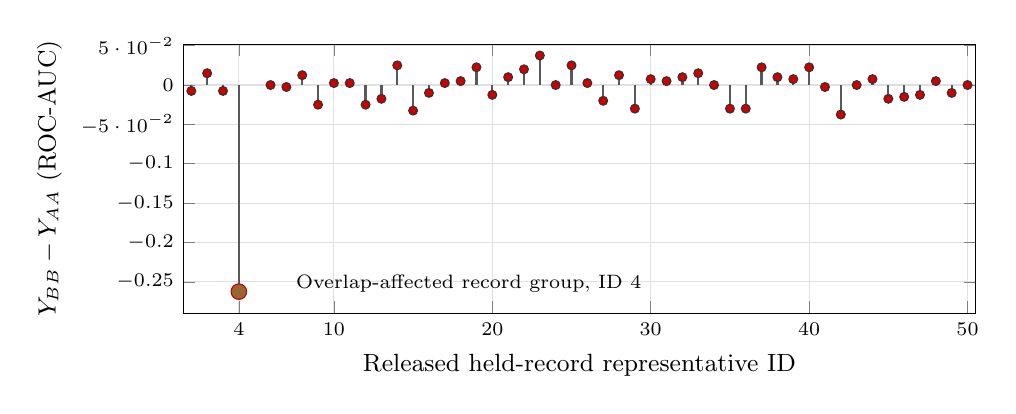
\begin{tikzpicture}
\begin{axis}[
 width=.96\linewidth,height=5.0cm,
 xmin=.5,xmax=50.5,ymin=-.29,ymax=.052,
 xtick={4,10,20,30,40,50},
 ytick={-.25,-.20,-.15,-.10,-.05,0,.05},
 xlabel={Released held-record representative ID},
 ylabel={$Y_{BB}-Y_{AA}$ (ROC-AUC)},
 grid=major,grid style={black!12},
 tick label style={font=\scriptsize},
 label style={font=\small},
 clip=false,
 ]
\addplot+[ycomb,no marks,thick,black!65]
 coordinates {(1,-0.0075) (2,0.0150) (3,-0.0075) (4,-0.2625) (6,0.0000) (7,-0.0025) (8,0.0125) (9,-0.0250) (10,0.0025) (11,0.0025) (12,-0.0250) (13,-0.0175) (14,0.0250) (15,-0.0325) (16,-0.0100) (17,0.0025) (18,0.0050) (19,0.0225) (20,-0.0125) (21,0.0100) (22,0.0200) (23,0.0375) (24,0.0000) (25,0.0250) (26,0.0025) (27,-0.0200) (28,0.0125) (29,-0.0300) (30,0.0075) (31,0.0050) (32,0.0100) (33,0.0150) (34,0.0000) (35,-0.0300) (36,-0.0300) (37,0.0225) (38,0.0100) (39,0.0075) (40,0.0225) (41,-0.0025) (42,-0.0375) (43,0.0000) (44,0.0075) (45,-0.0175) (46,-0.0150) (47,-0.0125) (48,0.0050) (49,-0.0100) (50,0.0000)};
\addplot+[only marks,mark=*,mark size=1.6pt,black!80]
 coordinates {(1,-0.0075) (2,0.0150) (3,-0.0075) (4,-0.2625) (6,0.0000) (7,-0.0025) (8,0.0125) (9,-0.0250) (10,0.0025) (11,0.0025) (12,-0.0250) (13,-0.0175) (14,0.0250) (15,-0.0325) (16,-0.0100) (17,0.0025) (18,0.0050) (19,0.0225) (20,-0.0125) (21,0.0100) (22,0.0200) (23,0.0375) (24,0.0000) (25,0.0250) (26,0.0025) (27,-0.0200) (28,0.0125) (29,-0.0300) (30,0.0075) (31,0.0050) (32,0.0100) (33,0.0150) (34,0.0000) (35,-0.0300) (36,-0.0300) (37,0.0225) (38,0.0100) (39,0.0075) (40,0.0225) (41,-0.0025) (42,-0.0375) (43,0.0000) (44,0.0075) (45,-0.0175) (46,-0.0150) (47,-0.0125) (48,0.0050) (49,-0.0100) (50,0.0000)};
\addplot+[only marks,mark=*,mark size=2.8pt,red!75!black]
 coordinates {(4,-0.2625)};
\node[anchor=west,font=\scriptsize] at (axis cs:7,-.252) {Overlap-affected record group, ID 4};
\end{axis}
\end{tikzpicture}
\caption{Real frozen 49-group paired full-change AUC values
under the original source-macro selection policy. The
single content-overlap-affected group (red marker)
shows a large local decrease after full content-disjoint
source refitting, whereas the other 48 groups have
mixed small gains/losses and a nearly zero average.
Each point is a \emph{processed content group}, not
an independently trained EEG model or a verified unique patient.
The plotted responses are previously exposed outcomes;
no new held target recordings or causal intervention
were introduced for this figure.}
\label{fig:p2-paired-49-localisation}
\end{figure}


\section{Discussion}
Our observation is more specific than generic random-window leakage:
the public released label unit was not enough to ensure disjoint
processed signal contents. The full data-integrity audit and two
independent-acquisition controls make the particular duplicate
verifiable and falsifiable, while the same-held-target factorial
prevents silently attributing the whole correction to a changing
regularisation parameter.

The source-macro policy changed $\lambda$ in 37/49 groups,
yet its two conditional source-model selector effects had
opposite signs. In contrast, neither the source-trained-mean
predictive Gaussian nor historical class-centred covariance
choice changed its $\lambda$ under this comparison. A changed
target mean could thus arise even with \emph{no}
regularisation-selection changes. These results separate
source-model dependence from parameter substitution, but do
not uniquely isolate causes of training contamination.

The overlap finding pertains to a fixed processed software
representation. Authoritative resolution of whether patient
records themselves were duplicated requires the original
data custodians and cannot be inferred from processed EEG.
All performance outcomes had been exposed before the V29
factorial and all apparent group-bootstrap intervals are
descriptive, not new confirmatory tests. This analysis does
not demonstrate a SOTA EEG decoder, a clinical outcome, or
a safety guarantee for unseen stroke patients. The
original Default Regularisation EEG estimand analysis
remains a separate primary paper and should not combine
these findings into its earlier frozen Holm families.

\section{Conclusion}
An EEG subject label is not automatically an independent
signal identity. Full processed epoch-content checks found
one complete cross-ID duplicate in a 50-ID acute-stroke
motor-imagery acquisition, and no exact cross-ID matches
in two preselected other acquisitions. A 49-recording-group
full refit and $2\times2$ frozen fit--selector contrast
showed that reporting weights, model fitting and source
selection must not be collapsed into a single asserted
leakage penalty. The practical implication is to audit
recording provenance before interpreting cross-subject
regularisation comparisons.

\section*{Statements and Declarations}
\textbf{Data and code availability:}
Liu2024, Weibo2014 and BNCI2014\_002 are publicly
distributed at their original repositories.
No EEG waveform recordings are redistributed here.
The implemented exact cross-ID content audit and
full source-refit study, with experiment protocol,
are available at
\url{https://github.com/lindicaphxag-tech/kaggle/pull/144}.
The original immutable 49-content-record full
factorial trial artifact and independent audit
are archived at
\url{https://github.com/lindicaphxag-tech/kaggle/actions/runs/38290349868}
and
\url{https://github.com/lindicaphxag-tech/kaggle/actions/runs/38315269388},
respectively. The manuscript is a source branch
research draft; a stable code/data release or DOI,
the public signal data use conditions, and
the complete author-approved disclosures
must be finalised before actual journal submission.\\
\textbf{Author, ethics, competing interests,
funding and AI-use statements:} to be verified by
the actual authors before submission; no claim is made
on anyone's behalf.

\bibliographystyle{unsrt}
\bibliography{references_v10}
\end{document}
